\documentclass[12pt,english,twoside]{report}
\usepackage[colorlinks,linkcolor=darkgray,urlcolor=darkgray]{hyperref}
%%\usepackage{chngcntr}
\usepackage{color}
\usepackage{float}
\usepackage{geometry}
\usepackage{graphicx}
\usepackage{longtable}
\usepackage{makecell}
\usepackage{makeidx}
\usepackage{times}
\IfFileExists{url.sty}{\usepackage{url}}
                      {\newcommand{\url}{\texttt}}
\usepackage{varioref}
                     
\renewcommand{\ttdefault}{cmtt}
\usepackage[T1]{fontenc}
\usepackage[latin1]{inputenc}

\definecolor{darkgray}{gray}{0.25}

\geometry{verbose,letterpaper,tmargin=1in,bmargin=1in,lmargin=1.25in,rmargin=1.25in,headheight=0in,headsep=0in,footskip=0.5in}
\setcounter{secnumdepth}{3}
\setcounter{tocdepth}{3}

\counterwithout{figure}{chapter}
\counterwithout{table}{chapter}

%%\makeindex
\makeatletter

\providecommand{\boldsymbol}[1]{\mbox{\boldmath $#1$}}
\def\code{\texttt}
\def\checkmark{\ensuremath{\times}}
\def\subsubsubsection{\paragraph}

\providecommand{\tabularnewline}{\\}
\floatstyle{ruled}
\newfloat{algorithm}{tbp}{loa}
\floatname{algorithm}{Algorithm}


\newcommand\incomplete[1]{{\color{red}\it #1}}
\newcommand\machineinst[1]{\hyperref[sec:Ins_#1]{\code{#1}}}
\newcommand\otc[3]{\hyperref[sec:Ins_#1]{\makecell{{\large \code{\textbf{#1}}}\\ {\small \textbf{#2}}}}}
\newcommand\otcinc[3]{\incomplete{\makecell{{\large \code{\textbf{#1}}}\\ {\small \textbf{#2}}}}}

\newenvironment{codeblock}
{\begin{list}{}{
\setlength{\rightmargin}{\leftmargin}
\setlength{\listparindent}{0pt}% needed for AMS classes
\raggedright
\setlength{\itemsep}{0pt}
\setlength{\parsep}{0pt}
\normalfont\ttfamily}%
 \item[]}
{\end{list}}

\newcommand\sectionname{Section}

\usepackage{babel}
\makeatother
\begin{document}

\title{\textbf{Omega CPU\\
Developers' Reference Manual}}


\author{August Schwerdfeger}


\date{Current to revision \code{db7bac7}}

\maketitle
\tableofcontents{}

\begin{abstract}
This manual contains documentation of the instruction-set architecture
and development tools of the Omega CPU, a 32-bit RISC processor
patterned after \href{https://en.wikipedia.org/wiki/MIPS_architecture#MIPS_I}{MIPS I}.

It is organized as follows. Chapter \ref{sec:ISA} describes the Omega
instruction-set architecture, including its register and memory model.
Chapter \ref{sec:Conventions} describes programming conventions for
the architecture, including those for procedure calls and interrupt
handling. Chapter \ref{sec:Assembler} describes the Omega assembler,
including several pseudo-instructions making use of the described
calling convention. Chapter \ref{sec:Implementations} describes the
existing implementations of the architecture.

As the Omega CPU is under active development, this manual may not
accurately reflect the latest changes in the architecture and/or
implementations. Documentation of incomplete features will be
annotated in type \incomplete{like this}.
\end{abstract}

\chapter{\label{sec:ISA} Instruction-set architecture.}

\section{Overview.}

\begin{table}[H]
\begin{tabular}{r|l}
  \textbf{Arithmetic} & Integer only, unsigned or two's complement\\
  \hline
  \textbf{Addressing mode} & Base + offset\\
  \hline
  \index{Endianness}\textbf{Endianness} & Little\\
  \hline
  \index{I/O}\textbf{I/O} & Port-mapped, 32 ports\\
  \hline
  \index{Instruction length}\textbf{Instruction length} & Fixed, 32 bits\\
  \hline
  \textbf{Max. operand count} & 4\\
  \hline
  \index{Memory model}\textbf{Memory model} & Flat, byte-addressable, 4 GiB max\\
                        & (absolute immediate jump limited to lower 256 MiB)\\
  \hline
  \textbf{Registers} & 1 constant\\
                     & 28 general-purpose\\
                     & 1 status\\
                     & 2 special-purpose\\
  \hline
  \index{Word size}\textbf{Word size} & 32 bits
  
\end{tabular}
\caption{\label{tab:Overview} Overview of Omega instruction-set architecture.}
\end{table}


\section{Registers.}

\index{Registers}The Omega architecture has 32 accessible registers,
numbered 0 through 31. All are 32 bits in size and of integer type.

\paragraph{Register 0.}
\index{Register 0}

Register 0 is a constant register with a fixed value of 0.

Instructions writing to register 0 are treated as no-ops.

\paragraph{Registers 1--28.}
Registers 1--28 are fully general-purpose registers (but see section
\ref{sec:RegisterUsage} for the purposes assigned to them by
convention).

\paragraph{Register 29.}
\index{Register 29}
Register 29 is a special-purpose register used to hold a return
address during interrupt handling (see section \ref{sec:Interrupts}).

Instructions may write to register 29.

\paragraph{Register 30.}
\index{Carry bit}\index{Status register}\index{Register 30}
Register 30 is a status register, with fields as follows:

\begin{itemize}
  \item \textbf{Bit 0: Carry bit.}\quad Following an add or subtract
    instruction, this bit will be 1 if the add or subtract operation
    overflowed, and 0 otherwise.
  \item \textbf{Bits 1--31: Unused.}
\end{itemize}

Instructions may write to register 30.

\paragraph{Register 31.}
\index{Program counter}\index{Register 31}
Register 31 is the program counter.

Instructions may write to register 31, but this is strongly discouraged.

\section{Memory model.}

The Omega architecture has a flat or linear memory model. Except for
an interrupt vector table (see section
\ref{sec:Interrupts}\incomplete{, but interrupt handling is
  incomplete}), the whole of memory is available for general-purpose
use.

The maximum amount of memory supported is the full 4 GiB allowed by a
32-bit address space. However, the absolute immediate jump instruction
(documented \vpageref{sec:Ins_JA}) holds its absolute address
in the 26-bit $I_A$ field. This gives only 28 effective address bits,
so this jump instruction cannot be used to jump to any address beyond
the lower 256 MiB. For absolute jumps to such addresses, the absolute
register jump must be used instead.

\section{Instruction set.}

\begin{table}[p]
  \begin{center}
  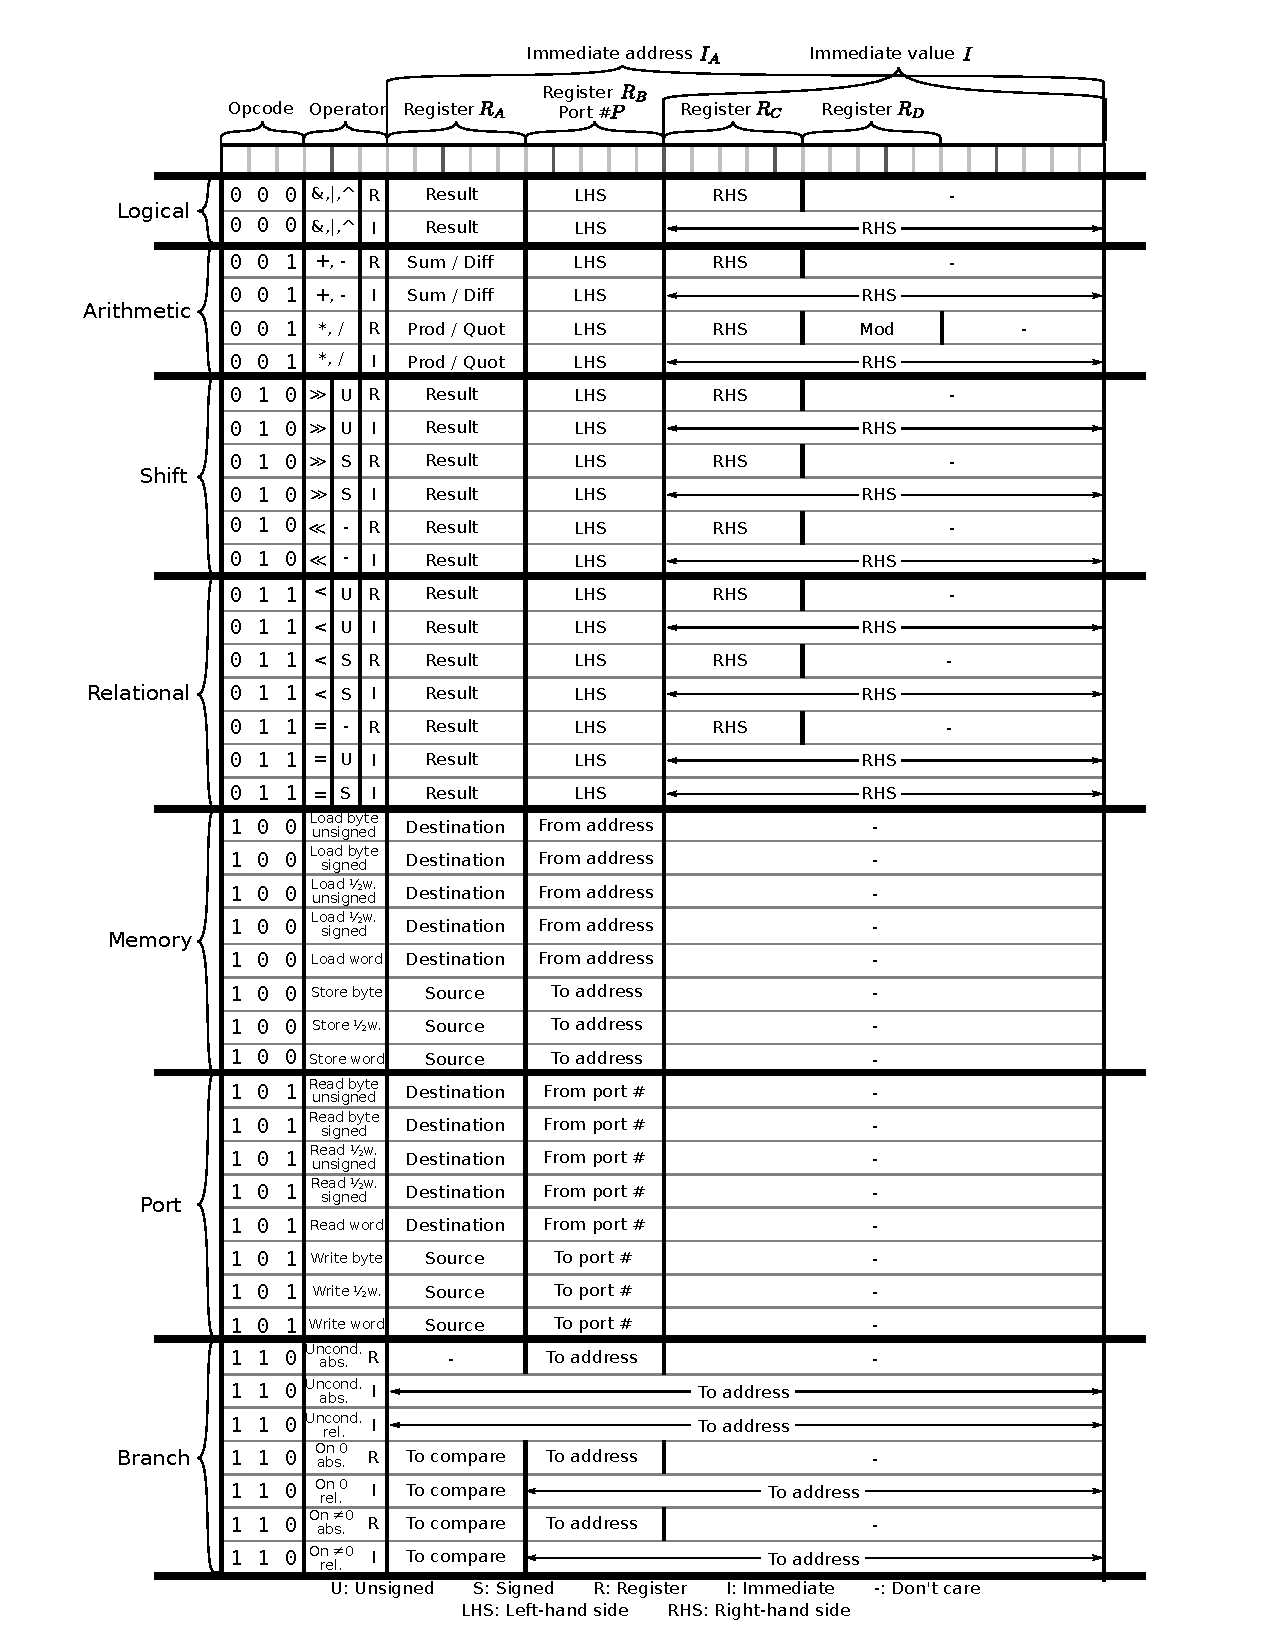
\includegraphics[width=6.5in]{../OmegaInstructionSet.pdf}
  \caption{\label{tab:OmegaInstructionSet} Instruction set.}
  \end{center}
\end{table}

See Table \ref{tab:OmegaInstructionSet} for a tabular representation
of all instructions in the Omega instruction set.

\subsection{Formats and fields.}

The Omega instruction set has a fixed instruction size of 32 bits, of
which the upper 6 are the opcode and the lower 26 hold any operands.
Depending on the specific \emph{format} of the instruction (see Table
\ref{tab:InstructionFormats} for a list of formats), the lower 26
bits will be interpreted as consisting of one or more of the
\emph{fields} delineated at the top of Table
\ref{tab:OmegaInstructionSet} (see Table \ref{tab:InstructionFields}
for a full list).

\begin{table}[p]
\begin{center}
\begin{tabular}{c|l}
  \textbf{Format} & \textbf{Operands}\\
  \hline
  \textbf{IA} & Immediate address only\\
  \hline
  \textbf{1R} & 1 register\\
  \hline
  \textbf{1R+IA} & 1 register and immediate address\\
  \hline
  \textbf{1R+P} & 1 register and 1 port number\\
  \hline
  \textbf{2R} & 2 registers\\
  \hline
  \textbf{2R+I} & 2 registers and immediate value\\
  \hline
  \textbf{3R} & 3 registers\\
  \hline
  \textbf{4R+M} & 4 registers and mode bit
\end{tabular}
\caption{\label{tab:InstructionFormats} Instruction formats.}
\end{center}
\end{table}

\begin{table}[p]
  \begin{center}
\begin{tabular}{c|c|l}
  \textbf{Field} & \textbf{Bit span} & \textbf{Description}\\
  \hline
  $DM$ & 0 & A bit used on divide instructions to select signed or unsigned mode.\\
  \hline
  $I$ & 15--0 & 16-bit immediate value field.\\
  \hline
  $I_A$ & 25--0 & 26-bit immediate address field for unconditional jumps.\\
  \hline
  $I_C$ & 20--0 & 21-bit immediate address field for conditional branches.\\
  \hline
  $P$ & 20--16 & 5-bit port number field, overlapping $R_B$.\\
  \hline
  $R_A$ & 25--21 & 5-bit register field.\\
  \hline
  $R_B$ & 20--16 & 5-bit register field.\\
  \hline
  $R_C$ & 15--11 & 5-bit register field.\\
  \hline
  $R_D$ & 10--6 & 5-bit register field.
\end{tabular}
\caption{\label{tab:InstructionFields} Operand fields.}
\end{center}
\end{table}

\begin{table}[p]
  \begin{center}
    \begin{tabular}{c||c|c|c|c|c|c|c|c|c}
      \makecell{Field$\rightarrow$ \\ $\downarrow$Format} & $DM$ & $I$ & $I_A$ & $I_C$ & $P$ & $R_A$ & $R_B$ & $R_C$ & $R_D$ \\
      \hline
      \textbf{IA} & & & \checkmark & & & & & &\\
      \hline
      \textbf{1R} & & & & & & & \checkmark & &\\
      \hline
      \textbf{1R+I} & & & & \checkmark & & \checkmark & & &\\
      \hline
      \textbf{1R+P} & & & & & \checkmark & \checkmark & & &\\
      \hline
      \textbf{2R} & & & & & & \checkmark & \checkmark & &\\
      \hline
      \textbf{2R+I} & & \checkmark & & & & \checkmark & \checkmark & &\\
      \hline
      \textbf{3R} & & & & & & \checkmark & \checkmark & \checkmark &\\
      \hline
      \textbf{4R+M} & \checkmark & & & & & \checkmark & \checkmark & \checkmark & \checkmark
    \end{tabular}
  \caption{\label{tab:FormatsAndFields} Which fields are used in which instruction formats.}
  \end{center}
\end{table}

\subsection{Instructions in detail.}

\begin{table}[p]
  \begin{center}
\begin{tabular}{c||c|c|c|c|c|c|c|c}
  \makecell{Operator$\rightarrow$ \\ $\downarrow$Opcode} & \textbf{000} & \textbf{001} & \textbf{010} & \textbf{011} & \textbf{100} & \textbf{101} & \textbf{110} & \textbf{111}\\
  \hline
  \textbf{000} & \otc{OR}{3R}{R_A,R_B,R_C} & \otc{ORI}{2R+I}{R_A,R_B,I} & \otc{AND}{3R}{R_A,R_B,R_C} & \otc{ANDI}{2R+I}{R_A,R_B,I} & \otc{XOR}{3R}{R_A,R_B,R_C} & \otc{XORI}{2R+I}{R_A,R_B,I} & \makecell{\emph{Invalid}\\ \emph{Instr.}} & \makecell{\emph{Invalid} \\ \emph{Instr.}} \\
  \hline
  \textbf{001} & \otc{ADD}{3R}{R_A,R_B,R_C} & \otc{ADDI}{2R+I}{R_A,R_B,I} & \otc{SUB}{3R}{R_A,R_B,R_C} & \otc{SUBI}{2R+I}{R_A,R_B,I} & \otc{MULT}{3R}{R_A,R_B,R_C} & \otc{MULTI}{2R+I}{R_A,R_B,I} & \otc{DIV}{4R+M}{DM,R_A,R_B,R_C,R_D} & \otc{DIVI}{2R+I}{R_A,R_B,I} \\
  \hline
  \textbf{010} & \otc{SRAV}{3R}{R_A,R_B,R_C} & \otc{SRA}{2R+I}{R_A,R_B,I} & \otc{SRLV}{3R}{R_A,R_B,R_C} & \otc{SRL}{2R+I}{R_A,R_B,I} & \otc{SLLV}{3R}{R_A,R_B,R_C} & \otc{SLL}{2R+I}{R_A,R_B,I} & \otcinc{SLLV}{3R}{R_A,R_B,R_C} & \otcinc{SLL}{2R+I}{R_A,R_B,I} \\
  \hline
  \textbf{011} & \otc{EQ}{3R}{R_A,R_B,R_C} & \otc{EQI}{2R+I}{R_A,R_B,I} & \otcinc{EQ}{3R}{R_A,R_B,R_C} & \otc{EQUI}{2R+I}{R_A,R_B,I} & \otc{LT}{3R}{R_A,R_B,R_C} & \otc{LTI}{2R+I}{R_A,R_B,I} & \otc{LTU}{3R}{R_A,R_B,R_C} & \otc{LTUI}{2R+I}{R_A,R_B,I} \\
  \hline
  \textbf{100} & \otc{LBU}{2R+I}{R_A,R_B,I} & \otc{LB}{2R+I}{R_A,R_B,I} & \otc{LHU}{2R+I}{R_A,R_B,I} & \otc{LH}{2R+I}{R_A,R_B,I} & \otc{LW}{2R+I}{R_A,R_B,I} & \otc{SB}{2R+I}{R_A,R_B,I} & \otc{SH}{2R+I}{R_A,R_B,I} & \otc{SW}{2R+I}{R_A,R_B,I} \\
  \hline
  \textbf{101} & \otc{INPBU}{1R+P}{R_A,P} & \otc{INPB}{1R+P}{R_A,P} & \otc{INPHU}{1R+P}{R_A,P} & \otc{INPH}{1R+P}{R_A,P} & \otc{INP}{1R+P}{R_A,P} & \otc{OUTPB}{1R+P}{R_A,P} & \otc{OUTPH}{1R+P}{R_A,P} & \otc{OUTP}{1R+P}{R_A,P} \\
  \hline
  \textbf{110} & \otc{JR}{1R}{R_B} & \otc{JA}{IA}{I_A} & \otc{J}{IA}{I_A} & \otc{BZ}{2R}{R_A,R_B} & \otc{BZI}{1R+I}{R_A,I_C} & \otc{BNZ}{2R}{R_A,R_B} & \otc{BNZI}{1R+I}{R_A,I_C} & \incomplete{\large \code{NOP}} \\
  \hline
  \textbf{111} & \incomplete{\makecell{\emph{Invalid} \\ \emph{Instr.}}} & \incomplete{\makecell{\emph{Invalid} \\ \emph{Instr.}}} & \incomplete{\makecell{\emph{Invalid} \\ \emph{Instr.}}} & \incomplete{\makecell{\emph{Invalid} \\ \emph{Instr.}}} & \incomplete{\makecell{\emph{Invalid} \\ \emph{Instr.}}} & \incomplete{\makecell{\emph{Invalid} \\ \emph{Instr.}}} & \incomplete{\makecell{\emph{Invalid} \\ \emph{Instr.}}} & \incomplete{\makecell{\emph{Invalid} \\ \emph{Instr.}}}
\end{tabular}
\caption{\label{tab:OpcodeTable}\index{Opcode table} Opcode table. Rows represent the opcode proper (upper 3 bits); columns, the operator (lower 3 bits). \incomplete{\code{SLLV}, \code{SLL}, and \code{EQ} have duplicate opcodes, marked in this typeface, that the assembler does not use, but that the implementations recognize.}}
\end{center}
\end{table}

\paragraph*{Terminology.} In this section, we describe the behavior of each instruction using snippets of pseudo-C. Some particulars of this notation:

\begin{itemize}
  \item System memory is represented as an array \code{mem}; registers
    and other operands as variables of the type as which they are
    treated during the instruction's operation.
  \item When converting a signed integer to a type of greater bit
    width (signed or unsigned), sign extension is performed. When converting
    unsigned integers, zero-filling is used.
  \item Integer variables may also be addressed as arrays of bits;
    \emph{e.g.} \code{var[7:0]} refers to the least significant byte
    of a word.
\end{itemize}

\subsubsection{Logical instructions.}

\subsubsubsection{\label{sec:Ins_OR}\code{OR}.}
\index{OR}\index{Inclusive OR}
Bitwise OR, register mode.

\begin{codeblock}
  uint32\_t $R_A$, $R_B$, $R_C$;
  
  $R_A$ = $R_B$ | $R_C$;
\end{codeblock}

\subsubsubsection{\label{sec:Ins_ORI}\code{ORI}.}
Bitwise OR, immediate mode.

\begin{codeblock}
  uint32\_t $R_A$, $R_B$;

  uint16\_t $I$;
  
  $R_A$ = $R_B$ | (uint32\_t) $I$;
\end{codeblock}

\subsubsubsection{\label{sec:Ins_AND}\code{AND}.}
\index{AND}
Bitwise AND, register mode.

\begin{codeblock}
  uint32\_t $R_A$, $R_B$, $R_C$;
  
  $R_A$ = $R_B$ \& $R_C$;
\end{codeblock}

\subsubsubsection{\label{sec:Ins_ANDI}\code{ANDI}.}
Bitwise AND, immediate mode.

\begin{codeblock}
  uint32\_t $R_A$, $R_B$;
  
  uint16\_t $I$;
  
  $R_A$ = $R_B$ \& (uint32\_t) $I$;
\end{codeblock}

\subsubsubsection{\label{sec:Ins_XOR}\code{XOR}.}
\index{XOR}\index{Exclusive OR}
Bitwise XOR, register mode.

\begin{codeblock}
  uint32\_t $R_A$, $R_B$, $R_C$;
  
  $R_A$ = $R_B$ \^{} $R_C$;
\end{codeblock}

\subsubsubsection{\label{sec:Ins_XORI}\code{XORI}.}
Bitwise XOR, immediate mode.

\begin{codeblock}
  uint32\_t $R_A$, $R_B$;

  uint16\_t $I$;
  
  $R_A$ = $R_B$ \^{} (uint32\_t) $I$;
\end{codeblock}

\subsubsection{Arithmetic instructions.}

\subsubsubsection{\label{sec:Ins_ADD}\code{ADD}.}
\index{Addition}
Addition, register mode.

\begin{codeblock}
  uint32\_t $R_A$, $R_B$, $R_C$;

  uint33\_t result = $R_B$ + $R_C$;

  $R_A$ = result[31:0];

  Carry = result[32];
\end{codeblock}

\subsubsubsection{\label{sec:Ins_ADDI}\code{ADDI}.}
Addition, immediate mode.

\begin{codeblock}
  uint32\_t $R_A$, $R_B$;

  int16\_t $I$;

  uint33\_t result = $R_B$ + (uint32\_t) $I$;

  $R_A$ = result[31:0];

  Carry = result[32];
\end{codeblock}

\subsubsubsection{\label{sec:Ins_SUB}\code{SUB}.}
\index{Subtraction}
Subtraction, register mode.

\begin{codeblock}
  uint32\_t $R_A$, $R_B$, $R_C$;

  uint33\_t result = $R_B$ - $R_C$;

  $R_A$ = result[31:0];

  Carry = result[32];
\end{codeblock}

\subsubsubsection{\label{sec:Ins_SUBI}\code{SUBI}.}
Subtraction, immediate mode.

\begin{codeblock}
  uint32\_t $R_A$, $R_B$;

  int16\_t $I$;

  uint33\_t result = $R_B$ - (uint32\_t) $I$;

  $R_A$ = result[31:0];

  Carry = result[32];
\end{codeblock}

\subsubsubsection{\label{sec:Ins_MULT}\code{MULT}.}
\index{Multiplication}
Multiplication, register mode.

\begin{codeblock}
  uint32\_t $R_A$, $R_B$, $R_C$;

  uint64\_t result = $R_B$ * $R_C$;

  $R_A$ = result[31:0];
\end{codeblock}

\subsubsubsection{\label{sec:Ins_MULTI}\code{MULTI}.}
Multiplication, immediate mode.

\begin{codeblock}
  uint32\_t $R_A$, $R_B$;

  int16\_t $I$;

  uint64\_t result = $R_B$ * (uint32\_t) $I$;

  $R_A$ = result[31:0];
\end{codeblock}

\subsubsubsection{\label{sec:Ins_DIV}\code{DIV}.}
\index{Division}
Division, register mode. It must be explicitly specified, using
the $DM$ bit, whether the operation should be signed or unsigned.

\begin{codeblock}
  
  bool $DM$;

  if($DM$) \{ // Signed mode

{}~~~~int32\_t $R_A$, $R_B$, $R_C$, $R_D$;
    
  \} else \{ // Unsigned mode
    
{}~~~~uint32\_t $R_A$, $R_B$, $R_C$, $R_D$;
    
  \}

  if($R_C$ == 0) \{

{}~~~~Status = DivideOverflow;

  \} else \{

{}~~~~$R_A$ = $R_B$ / $R_C$;

{}~~~~$R_D$ = $R_B$ \% $R_C$;
    
  \}
\end{codeblock}

\subsubsubsection{\label{sec:Ins_DIVI}\code{DIVI}.}
Division, immediate mode. This operates in signed mode only \incomplete{(but the implementation will set the mode according to the $DM$ bit)}.

\begin{codeblock}
  int32\_t $R_A$, $R_B$;

  int16\_t $I$;

  $R_A$ = $R_B$ / (int32\_t) $I$;
\end{codeblock}

\subsubsection{Shift instructions.}

\subsubsubsection{\label{sec:Ins_SRAV}\code{SRAV}.}
Shift right, arithmetic (sign-preserving), register mode.

\begin{codeblock}
  int32\_t $R_A$, $R_B$, $R_C$;

  $R_A$ = $R_B$ >{}> $R_C$;
\end{codeblock}

\subsubsubsection{\label{sec:Ins_SRA}\code{SRA}.}
Shift right, arithmetic (sign-preserving), immediate mode.

\begin{codeblock}
  int32\_t $R_A$, $R_B$;

  uint16\_t $I$;

  $R_A$ = $R_B$ >{}> $I$;
\end{codeblock}

\subsubsubsection{\label{sec:Ins_SRLV}\code{SRLV}.}
Shift right, logical (not sign-preserving), register mode.

\begin{codeblock}
  uint32\_t $R_A$, $R_B$, $R_C$;

  $R_A$ = $R_B$ >{}> $R_C$;
\end{codeblock}

\subsubsubsection{\label{sec:Ins_SRL}\code{SRL}.}
Shift right, logical (not sign-preserving), immediate mode.

\begin{codeblock}
  uint32\_t $R_A$, $R_B$;

  uint16\_t $I$;

  $R_A$ = $R_B$ >{}> $I$;
\end{codeblock}

\subsubsubsection{\label{sec:Ins_SLLV}\code{SLLV}.}
Shift left, register mode.

\begin{codeblock}
  uint32\_t $R_A$, $R_B$, $R_C$;

  $R_A$ = $R_B$ <{}< $R_C$;
\end{codeblock}

\subsubsubsection{\label{sec:Ins_SLL}\code{SLL}.}
Shift left, immediate mode.

\begin{codeblock}
  uint32\_t $R_A$, $R_B$;

  uint16\_t $I$;

  $R_A$ = $R_B$ <{}< $I$;
\end{codeblock}

\subsubsection{Relational instructions.}

\subsubsubsection{\label{sec:Ins_EQ}\code{EQ}.}
Equality test, register mode.

\begin{codeblock}
  uint32\_t $R_A$, $R_B$, $R_C$;

  if($R_B$ == $R_C$) \{

{}~~~~$R_A$ = 1;

  \} else \{

{}~~~~$R_A$ = 0;

  \}
\end{codeblock}

\subsubsubsection{\label{sec:Ins_EQI}\code{EQI}.}
Equality test, signed, immediate mode.

\begin{codeblock}
  uint32\_t $R_A$, $R_B$;

  int16\_t $I$;

  if($R_B$ == (uint32\_t) $I$) \{

{}~~~~$R_A$ = 1;

  \} else \{

{}~~~~$R_A$ = 0;

  \}
\end{codeblock}

\subsubsubsection{\label{sec:Ins_EQUI}\code{EQUI}.}
Equality test, unsigned, immediate mode.

\begin{codeblock}
  uint32\_t $R_A$, $R_B$;

  uint16\_t $I$;

  if($R_B$ == (uint32\_t) $I$) \{

{}~~~~$R_A$ = 1;

  \} else \{

{}~~~~$R_A$ = 0;

  \}
\end{codeblock}

\subsubsubsection{\label{sec:Ins_LT}\code{LT}.}
Inequality test, signed, register mode.

\begin{codeblock}
  uint32\_t $R_A$;

  int32\_t $R_B$, $R_C$;

  if($R_B$ < $R_C$) \{

{}~~~~$R_A$ = 1;

  \} else \{

{}~~~~$R_A$ = 0;

  \}
\end{codeblock}

\subsubsubsection{\label{sec:Ins_LTI}\code{LTI}.}
Inequality test, signed, immediate mode.

\begin{codeblock}
  uint32\_t $R_A$;

  int32\_t $R_B$;

  int16\_t $I$;

  if($R_B$ < (int32\_t) $I$) \{

{}~~~~$R_A$ = 1;

  \} else \{

{}~~~~$R_A$ = 0;

  \}
\end{codeblock}

\subsubsubsection{\label{sec:Ins_LTU}\code{LTU}.}
Inequality test, unsigned, register mode.

\begin{codeblock}
  uint32\_t $R_A$, $R_B$, $R_C$;

  if($R_B$ < $R_C$) \{

{}~~~~$R_A$ = 1;

  \} else \{

{}~~~~$R_A$ = 0;

  \}
\end{codeblock}

\subsubsubsection{\label{sec:Ins_LTUI}\code{LTUI}.}
Inequality test, unsigned, immediate mode.

\begin{codeblock}
  uint32\_t $R_A$, $R_B$;

  uint16\_t $I$;

  if($R_B$ < (uint32\_t) $I$) \{

{}~~~~$R_A$ = 1;

  \} else \{

{}~~~~$R_A$ = 0;

  \}
\end{codeblock}


\subsubsection{Load and store instructions.}

\subsubsubsection{\label{sec:Ins_LBU}\code{LBU}.}
Retrieve a byte from memory into a register, without sign extension.

\begin{codeblock}
  uint32\_t $R_A$;
  
  uint32\_t $R_B$;

  int16\_t $I$;

  uint32\_t addr = $R_B$ + (int32\_t) $I$;

  $R_A$ = (uint32\_t) mem[addr];
\end{codeblock}

\subsubsubsection{\label{sec:Ins_LB}\code{LB}.}
Retrieve a byte from memory into a register, with sign extension.

\begin{codeblock}
  uint32\_t $R_A$;
  
  uint32\_t $R_B$;

  int16\_t $I$;

  uint32\_t addr = $R_B$ + (int32\_t) $I$;

  $R_A$ = (int32\_t) mem[addr];
\end{codeblock}

\subsubsubsection{\label{sec:Ins_LHU}\code{LHU}.}
Retrieve a half-word from memory into a register, without sign extension.

\begin{codeblock}
  uint32\_t $R_A$;
  
  uint32\_t $R_B$;

  int16\_t $I$;

  uint32\_t addr = $R_B$ + (int32\_t) $I$;

  $R_A$[7:0] = mem[addr];

  $R_A$[31:8] = (uint24\_t) mem[addr + 1];
\end{codeblock}

\subsubsubsection{\label{sec:Ins_LH}\code{LH}.}
Retrieve a half-word from memory into a register, with sign extension.

\begin{codeblock}
  uint32\_t $R_A$;
  
  uint32\_t $R_B$;

  int16\_t $I$;

  uint32\_t addr = $R_B$ + (int32\_t) $I$;

  $R_A$[7:0] = mem[addr];

  $R_A$[31:8] = (int24\_t) mem[addr + 1];
\end{codeblock}

\subsubsubsection{\label{sec:Ins_LW}\code{LW}.}
Retrieve a word from memory into a register.

\begin{codeblock}
  uint32\_t $R_A$;
  
  uint32\_t $R_B$;

  int16\_t $I$;

  uint32\_t addr = $R_B$ + (int32\_t) $I$;

  $R_A$[7:0] = mem[addr];

  $R_A$[15:8] = mem[addr + 1];

  $R_A$[23:16] = mem[addr + 2];

  $R_A$[31:24] = mem[addr + 3];
\end{codeblock}

\subsubsubsection{\label{sec:Ins_SB}\code{SB}.}
Write a byte from a register into memory.

\begin{codeblock}
  uint32\_t $R_A$;

  uint32\_t $R_B$;

  int16\_t $I$;

  uint32\_t addr = $R_B$ + (int32\_t) $I$;

  mem[addr] = $R_A$[7:0];
\end{codeblock}

\subsubsubsection{\label{sec:Ins_SH}\code{SH}.}
Write a half word from a register into memory.

\begin{codeblock}
  uint32\_t $R_A$;

  uint32\_t $R_B$;

  int16\_t $I$;

  uint32\_t addr = $R_B$ + (int32\_t) $I$;

  mem[addr] = $R_A$[7:0];

  mem[addr + 1] = $R_A$[15:8];
\end{codeblock}

\subsubsubsection{\label{sec:Ins_SW}\code{SW}.}
Write a word from a register into memory.

\begin{codeblock}
  uint32\_t $R_A$;

  uint32\_t $R_B$;

  int16\_t $I$;

  uint32\_t addr = $R_B$ + (int32\_t) $I$;

  mem[addr] = $R_A$[7:0];

  mem[addr + 1] = $R_A$[15:8];

  mem[addr + 2] = $R_A$[15:8];

  mem[addr + 3] = $R_A$[15:8];
\end{codeblock}

\subsubsection{I/O instructions.}

\subsubsubsection{\label{sec:Ins_INPBU}\code{INPBU}.}
Read a byte from a port into a register, without sign extension.
\incomplete{This instruction may, at the discretion of the port
  controller, take an arbitrary amount of time to execute.}

\begin{codeblock}
  uint32\_t $R_A$;
  
  uint5\_t $P$;

  $R_A$ = (uint32\_t) inp($P$)[7:0];
\end{codeblock}

\subsubsubsection{\label{sec:Ins_INPB}\code{INPB}.}
Read a byte from a port into a register, with sign extension.
\incomplete{This instruction may, at the discretion of the port
  controller, take an arbitrary amount of time to execute.}

\begin{codeblock}
  uint32\_t $R_A$;
  
  uint5\_t $P$;

  $R_A$ = (int32\_t) inp($P$)[7:0];
\end{codeblock}

\subsubsubsection{\label{sec:Ins_INPHU}\code{INPHU}.}
Read a half-word from a port into a register, without sign extension.
\incomplete{This instruction may, at the discretion of the port
  controller, take an arbitrary amount of time to execute.}

\begin{codeblock}
  uint32\_t $R_A$;
  
  uint5\_t $P$;

  $R_A$ = (uint32\_t) inp($P$)[15:0];
\end{codeblock}

\subsubsubsection{\label{sec:Ins_INPH}\code{INPH}.}
Read a half-word from a port into a register, with sign extension.
\incomplete{This instruction may, at the discretion of the port
  controller, take an arbitrary amount of time to execute.}

\begin{codeblock}
  uint32\_t $R_A$;
  
  uint5\_t $P$;

  $R_A$ = (int32\_t) inp($P$)[15:0];
\end{codeblock}

\subsubsubsection{\label{sec:Ins_INP}\code{INP}.}
Read a word from a port into a register.
\incomplete{This instruction may, at the discretion of the port
  controller, take an arbitrary amount of time to execute.}

\begin{codeblock}
  uint32\_t $R_A$;
  
  uint5\_t $P$;

  $R_A$ = inp($P$);
\end{codeblock}

\subsubsubsection{\label{sec:Ins_OUTPB}\code{OUTPB}.}
Write a byte from a register to a port.

\begin{codeblock}
  uint32\_t $R_A$;

  uint5\_t $P$;

  outp($P$, (uint32\_t) $R_A$[7:0]);
\end{codeblock}

\subsubsubsection{\label{sec:Ins_OUTPH}\code{OUTPH}.}
Write a half word from a register to a port.

\begin{codeblock}
  uint32\_t $R_A$;

  uint5\_t $P$;

  outp($P$, (uint32\_t) $R_A$[15:0]);
\end{codeblock}

\subsubsubsection{\label{sec:Ins_OUTP}\code{OUTP}.}
Write a word from a register to a port.

\begin{codeblock}
  uint32\_t $R_A$;

  uint5\_t $P$;

  outp($P$, $R_A$);
\end{codeblock}


\subsubsection{Branch instructions.}

\subsubsubsection{\label{sec:Ins_JR}\code{JR}.}
Unconditional jump to an absolute address stored in a register.

\begin{codeblock}
  uint32\_t PC;

  uint32\_t $R_A$;

  PC = $R_A$;
\end{codeblock}

\subsubsubsection{\label{sec:Ins_JA}\code{JA}.}
Unconditional jump to an absolute immediate address.

\begin{codeblock}
  uint32\_t PC;

  int26\_t $I_A$;

  PC = (uint32\_t) ($I_A$ <{}< 2);
\end{codeblock}

\subsubsubsection{\label{sec:Ins_J}\code{J}.}
Unconditional jump to a relative immediate address.

\begin{codeblock}
  uint32\_t PC;

  int26\_t $I_A$;

  PC = PC + (int32\_t) ($I_A$ <{}< 2);
\end{codeblock}
  
\subsubsubsection{\label{sec:Ins_BZ}\code{BZ}.}
Branch on a zero condition to an absolute address stored in a register.

\begin{codeblock}
  uint32\_t PC;

  uint32\_t $R_A$, $R_B$;

  if($R_A$ == 0) \{

{}~~~~PC = $R_B$;

  \}
\end{codeblock}

\subsubsubsection{\label{sec:Ins_BZI}\code{BZI}.}
Branch on a zero condition to a relative immediate address.

\begin{codeblock}
  uint32\_t PC;

  uint32\_t $R_A$;

  int21\_t $I_C$;

  if($R_A$ == 0) \{

{}~~~~PC = PC + (int32\_t) ($I_C$ <{}< 2);

  \}
\end{codeblock}

\subsubsubsection{\label{sec:Ins_BNZ}\code{BNZ}.}
Branch on a nonzero condition to an absolute address stored in a register.

\begin{codeblock}
  uint32\_t PC;

  uint32\_t $R_A$, $R_B$;

  if($R_A$ != 0) \{

{}~~~~PC = $R_B$;

  \}
\end{codeblock}

\subsubsubsection{\label{sec:Ins_BNZI}\code{BNZI}.}
Branch on a nonzero condition to a relative immediate address.

\begin{codeblock}
  uint32\_t PC;

  uint32\_t $R_A$;

  int21\_t $I_C$;

  if($R_A$ != 0) \{

{}~~~~PC = PC + (int32\_t) ($I_C$ <{}< 2);

  \}
\end{codeblock}

\chapter{\label{sec:Conventions} Conventions and implementation details.}

\section{\label{sec:CallingConvention} Calling convention.}
\index{Calling convention} The calling convention implemented by the
Omega assembler is patterned after the
\href{https://en.wikipedia.org/wiki/Calling_convention#MIPS}{O32
  convention} used with MIPS.

\subsection{\label{sec:RegisterUsage} Register usage.}

Table \ref{tab:CallingConventionRegisters} shows the designated
purpose of registers under the calling convention.

\begin{table}[h]
  \begin{center}
  \begin{tabular}{c|c|c|c}
    \textbf{Register} & \textbf{Purpose} & \makecell{\textbf{Must be preserved}\\ \textbf{through call}} & \makecell{\textbf{Programs should}\\ \textbf{use directly}}\\
    \hline
    1 & Assembler temporary & No & \textbf{No} \\
    \hline
    2,3 & Return values 0,1 & No & Yes \\
    \hline
    4--7 & Parameters 0--3 & No & Yes \\
    \hline
    8--15 & General purpose (volatile) & No & Yes \\
    \hline
    16--23 & General purpose (static) & \textbf{Yes} & Yes \\
    \hline
    24--26 & General purpose (volatile) & No & Yes \\
    \hline
    27 & \index{Stack pointer} Stack pointer & \textbf{Yes} & Yes \\
    \hline
    28 & \index{Frame pointer} Frame pointer & \textbf{Yes} & Read only \\
    \hline
    29 & \index{Return address register} Return address & No & \textbf{No} \\
    \hline
    30 & Status register & No & Read only \\
    \hline
    31 & Program counter & No & \textbf{No}
  \end{tabular}
  \end{center}
  \caption{\label{tab:CallingConventionRegisters} How registers are used in the Omega calling convention; whether a called routine must leave them as found, and whether assembly-language programs should reference them directly.}
\end{table}

\subsection{Stack structure and protocols.}

The stack in the Omega calling convention grows downward from any
selected address. Both the stack and frame pointers (registers 27 and
28, respectively) are set to this address to start.

A push is performed by storing the new element to the location
indicated by the stack pointer, then decrementing the stack pointer by
4. A pop is performed by incrementing the stack pointer by 4.

A new stack frame is created by pushing the value of the frame pointer
and then the value of the return address register (register 29). The
frame pointer is then set to point at the stack element containing its
former value. When the stack frame is destroyed, these two values are
popped and restored to their respective registers.

The exact mechanisms by which this convention is implemented are
detailed in section \ref{sec:Assembler}, in the documentation of the
assembler's \hyperref[Asm_CALL]{\code{CALL}} and
\hyperref[Asm_RET]{\code{RET}} pseudo-instructions.

\section{\label{sec:Interrupts} Interrupt handling.}

Although the specific details of interrupt handling are left to
implementations\incomplete{ (and are incomplete)}, this is the common
behavior to be followed by all implementations.

There is a section of memory designated as the interrupt vector table.
This may begin at any memory address $IV_0$ chosen by the
implementation, and will consist of as many words as there are
available interrupts. Each interrupt will be given a unique numeric
designator, greater than or equal to 1.

Before executing each instruction, the processor will check if any
interrupts have been received and not serviced, and if so will service
the one with the lowest number, $n$.

In servicing an interrupt, the processor will first load the contents
of memory location $IV_0 + 4n$. If it is equal to 0, no action
will be taken. But if it is non-zero, the current value of the program
counter will be written to register 29 and the value at memory
location $IV_0 + 4n$ will be written to the program counter.

Thereafter, no more interrupts will be serviced until after the
processor executes a \machineinst{JR} instruction with register 29 as
the operand. This instruction is meant to be rendered in the assembler
using the \code{RET} pseudo-instruction (see page \pageref{Asm_RET}).

\chapter{\label{sec:Assembler} Assembler.}
\index{Python}

The Omega assembler is a Python-language cross-assembler with syntax
derived from that of the MIPS assembly language.

\section{Command-line interface.}

The assembler may be invoked from the command line as follows:

\begin{codeblock}
  \$ python OmegaAssembler.py asm\_1.s asm\_2.s ... asm\_n.s > out.bin
\end{codeblock}

This will concatenate all the input files (\code{asm\_1.s} through
\code{asm\_n.s}) into one string, in command-line order. This string
is then assembled and the resulting machine code sent to standard
output.

\section{Syntax overview.}

Each assembly-language file consists of zero or more lines.

A line may be blank (whitespace only), a comment (beginning with a
hash symbol), an instruction, or a directive. Lines containing instructions
and directives generally begin with a tab character.

Any line (blank or not) may be prepended with one or more alphanumeric
labels. Labels must start with a letter or underscore; contain only
letters, numbers, underscores, and periods; and be suffixed with a
colon. Each label will be assigned the address of the most closely
following data-directive or instruction (see section
\ref{sec:AddressAssignment} for details on address assignment).

For example, in the following snippet, the labels \code{foo} and
\code{bar} will both be assigned the address of the add instruction:

\begin{codeblock}
  {}~~~~J foo
  
  {}~~~~J bar
  
  foo:

  bar: ADD \$r1,\$r2,\$r3
\end{codeblock}

Instructions and directives consist of an opcode or directive name
followed by one or more operands. All supported operand types are shown
in Table \ref{tab:AssemblerOperands}.

\begin{table}[h]
  \begin{center}
\begin{tabular}{c|c|c}
  \textbf{Operand type} & \textbf{Syntax} & \textbf{Matches regex}\\
  \hline
  Immediate value & Signed decimal integer & \code{[-]?(0|[1-9][0-9]*)}\\
  \hline
  Label reference & Name of label & \code{[A-Za-z\_][A-Za-z\_.0-9]}\\
  \hline
  Port reference & \code{\$p}$n$ & N/A \\
  \hline
  Register reference & \code{\$r}$n$ & N/A \\
  \hline
  \makecell{String literal\\ (\code{.asciiz} directive only)} & Python-syntax string & N/A\\
  \hline
\end{tabular}
\caption{\label{tab:AssemblerOperands} Operand types supported by the Omega assembler.}
  \end{center}
\end{table}

\section{\label{sec:AddressAssignment} Address assignment and output format.}

Each instruction and data directive in the input is assigned a memory
address where its corresponding machine code will be placed.

By default, the first instruction or data-directive in the input will
be assigned to memory address 0, while each subsequent
instruction/data-directive will be assigned to the next (word-aligned)
address following its immediate predecessor. However, the
\hyperref[Asm_data]{\code{.data}} and
\hyperref[Asm_text]{\code{.text}} directives may specify an address
explicitly.

The output of the assembler is a series of lines, each a 32-bit binary
number representing a word of memory in canonical form (\emph{i.e.},
the sequence of four bytes in each word must be reversed to produce
the actual order they will take in memory). The sequence starts at
address 0 and progresses as high as necessary: line $n$ corresponds to
memory address $4\cdot(n-1)$.

\section{Directives and instructions.}

\subsection{Machine instructions.}

The majority of Omega assembler instructions correspond exactly with
machine instructions and are assembled into a single machine
instruction (4 bytes in size), with some minor changes, as detailed below:

  \begin{center}
    \begin{longtable}{l|l}
      \textbf{Assembler instruction} & \textbf{Machine instruction}\\
      \hline
      \code{OR $R_A$,$R_B$,$R_C$} & \machineinst{OR}\\
      \hline
      \code{ORI $R_A$,$R_B$,$I$} & \machineinst{ORI}\\
      \hline
      \code{AND $R_A$,$R_B$,$R_C$} & \machineinst{AND}\\
      \hline
      \code{ANDI $R_A$,$R_B$,$I$} & \machineinst{ANDI}\\
      \hline
      \code{XOR $R_A$,$R_B$,$R_C$} & \machineinst{XOR}\\
      \hline
      \code{XORI $R_A$,$R_B$,$I$} & \machineinst{XORI}\\
      \hline
      \code{ADD $R_A$,$R_B$,$R_C$} & \machineinst{ADD}\\
      \hline
      \code{ADDI $R_A$,$R_B$,$I$} & \machineinst{ADDI}\\
      \hline
      \code{SUB $R_A$,$R_B$,$R_C$} & \machineinst{SUB}\\
      \hline
      \code{SUBI $R_A$,$R_B$,$I$} & \machineinst{SUBI}\\
      \hline
      \code{MULT $R_A$,$R_B$,$R_C$} & \machineinst{MULT}\\
      \hline
      \code{MULTI $R_A$,$R_B$,$I$} & \machineinst{MULTI}\\
      \hline
      \code{DIV $R_A$,$R_B$,$R_C$} & \machineinst{DIV} with $DM$ = 1\\
      \hline
      \code{DIVU $R_A$,$R_B$,$R_C$} & \machineinst{DIV} with $DM$ = 0\\
      \hline
      \code{DIVI $R_A$,$R_B$,$I$} & \machineinst{DIVI}\\
      \hline
      \code{SRAV $R_A$,$R_B$,$R_C$} & \machineinst{SRAV}\\
      \hline
      \code{SRA $R_A$,$R_B$,$I$} & \machineinst{SRA}\\
      \hline
      \code{SRLV $R_A$,$R_B$,$R_C$} & \machineinst{SRLV}\\
      \hline
      \code{SRL $R_A$,$R_B$,$I$} & \machineinst{SRL}\\
      \hline
      \code{SLLV $R_A$,$R_B$,$R_C$} & \machineinst{SLLV}\\
      \hline
      \code{SLL $R_A$,$R_B$,$I$} & \machineinst{SLL}\\
      \hline
      \code{EQ $R_A$,$R_B$,$R_C$} & \machineinst{EQ}\\
      \hline
      \code{EQI $R_A$,$R_B$,$I$} & \machineinst{EQI}\\
      \hline
      \code{EQUI $R_A$,$R_B$,$I$} & \machineinst{EQUI}\\
      \hline
      \code{LT $R_A$,$R_B$,$R_C$} & \machineinst{LT}\\
      \hline
      \code{LTI $R_A$,$R_B$,$I$} & \machineinst{LTI}\\
      \hline
      \code{LTU $R_A$,$R_B$,$R_C$} & \machineinst{LTU}\\
      \hline
      \code{LTUI $R_A$,$R_B$,$I$} & \machineinst{LTUI}\\
      \hline
      \code{LBU $R_A$,$R_B$[,$I$]} & \machineinst{LBU} ($I$ = 0 if omitted)\\
      \hline
      \code{LB $R_A$,$R_B$[,$I$]} & \machineinst{LB} ($I$ = 0 if omitted)\\
      \hline
      \code{LHU $R_A$,$R_B$[,$I$]} & \machineinst{LHU} ($I$ = 0 if omitted)\\
      \hline
      \code{LH $R_A$,$R_B$[,$I$]} & \machineinst{LH} ($I$ = 0 if omitted)\\
      \hline
      \code{LW $R_A$,$R_B$[,$I$]} & \machineinst{LW} ($I$ = 0 if omitted)\\
      \hline
      \code{SB $R_A$,$R_B$[,$I$]} & \machineinst{SB} ($I$ = 0 if omitted)\\
      \hline
      \code{SH $R_A$,$R_B$[,$I$]} & \machineinst{SH} ($I$ = 0 if omitted)\\
      \hline
      \code{SW $R_A$,$R_B$[,$I$]} & \machineinst{SW} ($I$ = 0 if omitted)\\
      \hline
      \code{INPBU $R_A$,$P$} & \machineinst{INPBU}\\
      \hline
      \code{INPB $R_A$,$P$} & \machineinst{INPB}\\
      \hline
      \code{INPHU $R_A$,$P$} & \machineinst{INPHU}\\
      \hline
      \code{INPH $R_A$,$P$} & \machineinst{INPH}\\
      \hline
      \code{INP $R_A$,$P$} & \machineinst{INP}\\
      \hline
      \code{OUTPB $R_A$,$P$} & \machineinst{OUTPB}\\
      \hline
      \code{OUTPH $R_A$,$P$} & \machineinst{OUTPH}\\
      \hline
      \code{OUTP $R_A$,$P$} & \machineinst{OUTP}\\
      \hline
      \code{JR $R_A$} & \machineinst{JR}\\
      \hline
      \code{JA $\mathit{label}$} & \machineinst{JA} with $I_A$ = absolute addr. of $\mathit{label}$\\
      \hline
      \code{J $\mathit{label}$} & \machineinst{J} with $I_A$ = relative addr. of $\mathit{label}$\\
      \hline
      \code{BZ} $R_A$,$R_B$ & \machineinst{BZ}\\
      \hline
      \code{BZI} $R_A$,$\mathit{label}$ & \machineinst{BZI} with $I_C$ = relative addr. of $\mathit{label}$\\
      \hline
      \code{BNZ} $R_A$,$R_B$ & \machineinst{BNZ}\\
      \hline
      \code{BNZI} $R_A$,$\mathit{label}$ & \machineinst{BNZI} with $I_C$ = relative addr. of $\mathit{label}$\\
      \hline
    \end{longtable}
  \end{center}
  
\subsection{Pseudo-instructions.}

There are three Omega assembler instructions that do not correspond to
any machine instruction, and are assembled into more than one machine
instruction.

Programs using any of these pseudo-instructions are expected to follow
the conventions for register usage detailed in Table
\ref{tab:CallingConventionRegisters}.

\subsubsection*{\label{Asm_LA} \code{LA}.}
\paragraph{Form.} \code{LA $R$, $\mathit{label}$}

\paragraph{Assembled length.} 28 bytes.

\paragraph{Function.} Load the absolute address of $\mathit{label}$ into
the register $R$.

\paragraph{Machine code.}
If the address of $\mathit{label}$ is held in a 32-bit integer
\code{addr}, the pseudo-instruction \code{LA $R$,$\mathit{label}$} is
converted to the following machine code:

\begin{codeblock}
  ADDI $R$,\$r0,addr[31:24]
  
  SLL $R$,$R$,8

  ADDI $R$,$R$,addr[23:16]

  SLL $R$,$R$,8

  ADDI $R$,$R$,addr[15:8]

  SLL $R$,$R$,8

  ADDI $R$,$R$,addr[7:0]
\end{codeblock}

\subsubsection*{\label{Asm_CALL} \code{CALL}.}
\paragraph{Form.} \code{CALL $\mathit{label}$}

\paragraph{Assembled length.} 44 bytes.

\paragraph{Function.} Call a subroutine, according to the calling convention detailed above.

\paragraph{Machine code.}
If the address of $\mathit{label}$ is held in a 26-bit integer
\code{addr}, the pseudo-instruction \code{CALL $\mathit{label}$} is
converted to the following machine code:

\begin{codeblock}
  SW \$r28,\$r27
  
  ADDI \$r28,\$r27,0
  
  SUBI \$r27,\$r27,4
  
  SW \$r29,\$r27
  
  SUBI \$r27,\$r27,4
  
  ADDI \$r29,\$r31,4
  
  J addr
  
  SUBI \$r27,\$r28,4
  
  LW \$r29,\$r27
  
  ADDI \$r27,\$r27,4
  
  LW \$r28,\$r27
\end{codeblock}

\subsubsection*{\label{Asm_RET} \code{RET}.}
\paragraph{Form.}
\code{RET} (no operands)

\paragraph{Assembled length.} 4 bytes.

\paragraph{Function.}
Return from a function called according to the calling convention
detailed above.

\paragraph{Machine code.}
A \code{RET} pseudo-instruction translates to a single machine
instruction:

\begin{codeblock}
  JR \$r29
\end{codeblock}

\subsection{Directives.}

\subsubsection*{\label{Asm_asciiz}\code{.asciiz}.}
\paragraph{Form.}
\code{.asciiz $\mathit{string}$}

\paragraph{Assembled length.} String length + 1.

\paragraph{Function.}
Put a null-terminated ASCII string at the designated location in
memory. The parameter is parsed within the assembler as a Python
string literal and supports all escape sequences.

\subsubsection*{\label{Asm_byte}\code{.byte}.}
\paragraph{Form.}
\code{.byte $I$\{,$I$\}}

\paragraph{Assembled length.} Number of operands.

\paragraph{Function.}
Put one or more data bytes at the designated location in memory, in
the exact order given. The numbers must be in decimal form and in the
range 0 to 255.

\subsubsection*{\label{Asm_data}\code{.data}.}
\paragraph{Form.}
\code{.data [$I$]}

\paragraph{Assembled length.} N/A.

\paragraph{Function.}
Indicates the start of a data segment. If the operand $I$ is
provided\incomplete{ (but this does not work)}, the segment will start
  at the given address\incomplete{ (or the next higher multiple
    of 4)}.

\subsubsection*{\label{Asm_text}\code{.text}.}
\paragraph{Form.}
\code{.text [$I$]}

\paragraph{Assembled length.} N/A.

\paragraph{Function.}
Indicates the start of a code segment. If the operand $I$ is provided,
the segment will start at the given address\incomplete{ (or the next
  higher multiple of 4)}.

\chapter{\label{sec:Implementations} Implementations.}

\section{Papilio Duo FPGA board.}

%% Division is implemented using the ``slow non-restoring'' algorithm.

\section{Emulation in GHDL.}

\section{Emulation in software.}

%\addcontentsline{toc}{chapter}{Index}
%\printindex{}

\end{document}
